\documentclass{article}
\usepackage[colorlinks=true]{hyperref}
\usepackage{geometry}
\usepackage{fancyhdr}
\usepackage{palatino}
\usepackage{titlesec}
\usepackage{pbox}
\usepackage{multicol}
\usepackage{graphicx}
\usepackage{enumitem}

\renewcommand{\baselinestretch}{1.15}
\geometry{margin=1in}
\geometry{headheight=2in}
\geometry{top=2in}
\titlespacing\section{0pt}{12pt plus 2pt minus 2pt}{0pt plus 2pt minus 2pt}
\lhead{}
\rhead{}
\pagestyle{fancy}
\setlength{\parskip}{0.5em}
\date{\today}

\title{CS 145 Milestone 1 - ToMEto}
\author{Jonathan Joo, Matthew Jin, Boyu (Charlie) Tong, Albert Ge}
\chead{%
  {\vbox{%
      \vspace{2mm}
      \large
      Networks: Structure Economics \hfill
      Caltech CMS/CS/EE 145 \hfill \\[1pt]
      CS 145 Milestone 1 - ToMEto \hfill
      \date{\today} \\
    }
  }
}

% \linespread{1.5}


\begin{document}
\maketitle

\section{Goals}
As per our project plan, the two early milestones we wanted to accomplish were:
\begin{enumerate}
    \item Begin data collecting
    \item Set up storate environments
\end{enumerate}

On the specifics of the milestones, these past two weeks we planned on familiarizing ourselves with the environment, i.e.
looking at APIs, figuring out which websites to crawl. Additionally, as per last week's meeting, we set out to investigate
\begin{enumerate}
    \item More of the literature regarding recipe recommendations
    \item Existing recipe applications
    \item Obtain data quickly, either by scraping ourselves or asking others
\end{enumerate}

\section{Progress}

\subsection{Existing applications}
There are several recipe apps, but not many of them are set out to
discover new ingredient combinations. Many
recipe apps are meant to be primarily used as a "recipe management
system"; step-by-step recipe instructions, cooking tips, saving
favorited recipes and suggesting (already existing) recipes
based on the ones you have favorited, and so on. \\ 
Of the ones that appear to be the most novel and are
not just a database for recipes, there are:
\begin{enumerate}
    \item Yummly - a user inputs dietary restrictions/tastes
        to find recipes that are tailored to those constraints
    \item Tender - similar interface as \textit{Tinder}:
        the user can swipe left or right on the shown recipe,
        and recommended recipes are filtered by swipe choices
\end{enumerate}

There are also a number of food pairing apps, but a majority
of these are merely food-and-wine pairings, not necessarily
food-and-food suggestions. Such an example is Pair It!,
which is a subscription-based service that provides 
recommendations on wine that would pair with a particular
cheese or other solid ingredient.

One particular contender is \texttt{http://www.foodpairing.com},
which is perhaps the closest in terms of the end case that
we wish to accomplish. The approach however, appears to
be much more at a molecular level: they use laboratory techniques
to categorize ingredients exactly by molecular composition,
and determine pairings by looking at combinations 
or different molecular aromas. This website
appears to be geared towards chefs; a quick glimpse
at their blog, for example, lists pairings between
ingredients that are not commonplace and the preparation
is incredibly detailed.




\subsection{Literature}

Much of the existing literature uses machine-learning techniques to make
recommendations, rate recipes, or make suggestions about substituting ingredients, and due to our limited knowledge
in this field, it is not a path we wish to pursue much further. Consequently, we refine our search for simpler
food-related papers. Before we decided on a use case, we perused through a variety of articles, some of which
we list and reflect on below: \\

\begin{enumerate}
    \item \textbf{Recipe recommendation using ingredient
        networks:} \texttt{http://dl.acm.org/citation.cfm?id=2380757} \\
        This was the original paper that was our inspiration. The authors
        scrape allrecipes.com, gathering not only recipes with their
        ingredients, but user reviews as well. Using machine learning
        techniques and also some network specific tools, such as centrality
        measures, they create a rating system for lists of ingredients.
        They are able to accurately predict user preference not using a
        full list of ingredients, but by using the relationship between
        ingredients, indicating there is a significant underlying network
        effect in play here.

    \item
    \textbf{Personalized recipe for healthy choices:} \texttt{http://dl.acm.org/citation.cfm?id=1943487} \\
    This describes a prototype for personalizing recipes such that the result returned to the user
    is nutritious and healthy. This allows the user to specify down to the nutrient level (e.g. vitamins and fibers),
    and takes information about the user's past meal choices. This could
    be something to look further into but there exist a plethora of
    websites and applications that offer healthy alternatives to
    certain ingredients in recipes, and often the ``tastiness'' of the
    recipe is very subjective, so for the moment healthiness of a recipe
    is not a use case we'd like to pursue.

    \textbf{Geography and Similarity of Regional Cuisines in China} \\
    \texttt{http://journals.plos.org/plosone/article?id=10.1371\%2Fjournal.pone.0079161}.
    This is a paper about identifying and explaining how different cuisines
    in China arose from regional differences in China. They scraped
    \texttt{http://www.meishij.net}, which is a site that categorizes
    chinese recipes by regions. Their main finding was that
    regions with similar cuisines were more geographically close,
    as opposed to having similar climates. Here they used the
    Pearson correlation coefficient to determine linearity
    between two sets of vectors (e.g., a vector of recipes,
    and a vector of ingredients). The analysis may be
    worth looking into, because it will help us better
    understand how to quantify the similarities between
    a set of ingredients.

\end{enumerate}

\subsection{Use case}
Because recipe suggestion appears to be largely based on machine-learning, we turned instead
our attention a use case that relies less on recommendations, and looks into how
food is represented as a graph, and the connections between different ingredients. In particular,
we have currently decided to focus on utilizing \textit{fusion of cuisines}, given that
particular ingredients may be cross-utilized in different regions. Therefore, our use case is to:
\begin{enumerate}
    \item User inputs what fusion cuisine they desire
    \item Result returns a recipe that is from one cuisine, but contains substituted ingredients that
        exist in a second cuisine, thereby creating a fusion dish
\end{enumerate}


\subsection{Data collection \& storage}
We have begun acquiring data from online recipe sources, namely \texttt{http://cooking.nytimes.com} and \texttt{http://allrecipes.com} because their sites make it easy to extract the list of ingredients. We wrote scrapers that crawl the websites, collecting recipe webpages and saving them locally as html/text files. Right now we are downloading recipes at about 1000 per hour from each website. We employ a sleep timer to slow down downloads and avoid being throttled.

For parsing the data, we wrote scripts that employ regex that extract the ingredients from each recipe webpage. Right now the data is still stored locally in text files. In the upcoming week, we will work on postprocessing the ingredients list. One specific task that needs to be done is removing the quantifiers (1 cup, 1 tablespoon, etc.) from the \texttt{http://allrecipes.com} recipes. The \texttt{http://cooking.nytimes.com} recipes have quantifiers separate, so not much postprocessing needs to be done for them.


\subsection{Front-end APIs}
For front-end, we were able to get some baseline code up and running for our website. We currently have two pages, a landing page and then a page that allows you to enter up to ten ingredients. Upon pressing a button, these ingredients are then sent to app.py, which is a python script which will likely handle all of the algorithms with this information. The ingredients are conveniently stored in an array, so that our backend can use these inputs to determine which ingredients to generate.

The following sites were useful in creating this website, which is fully interactive and usable right now.
\begin{itemize}
\item http://code.tutsplus.com/tutorials/creating-a-web-app-from-scratch-using-python-flask-and-mysql--cms-22972
\item http://www.randomsnippets.com/2008/02/21/how-to-dynamically-add-form-elements-via-javascript/
\end{itemize}

Here is a screenshot of our landing page: \\
\begin{center}
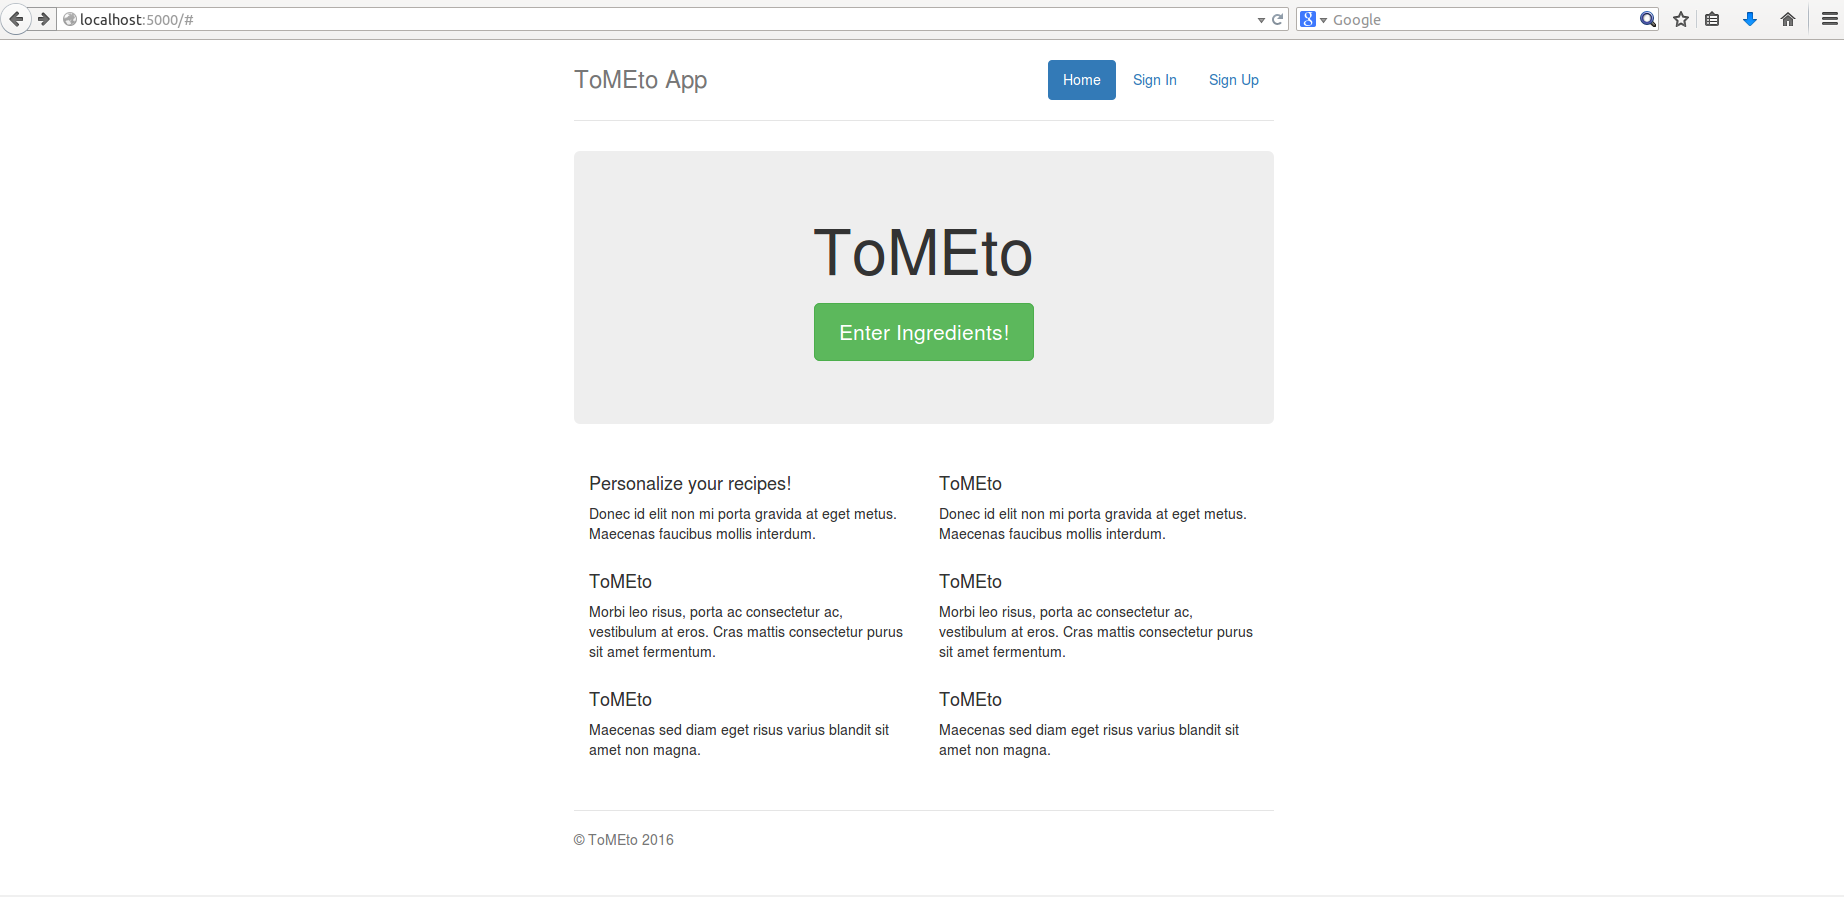
\includegraphics[scale=0.4]{firstpage.PNG}
\end{center}

And our submission page: \\
\begin{center}
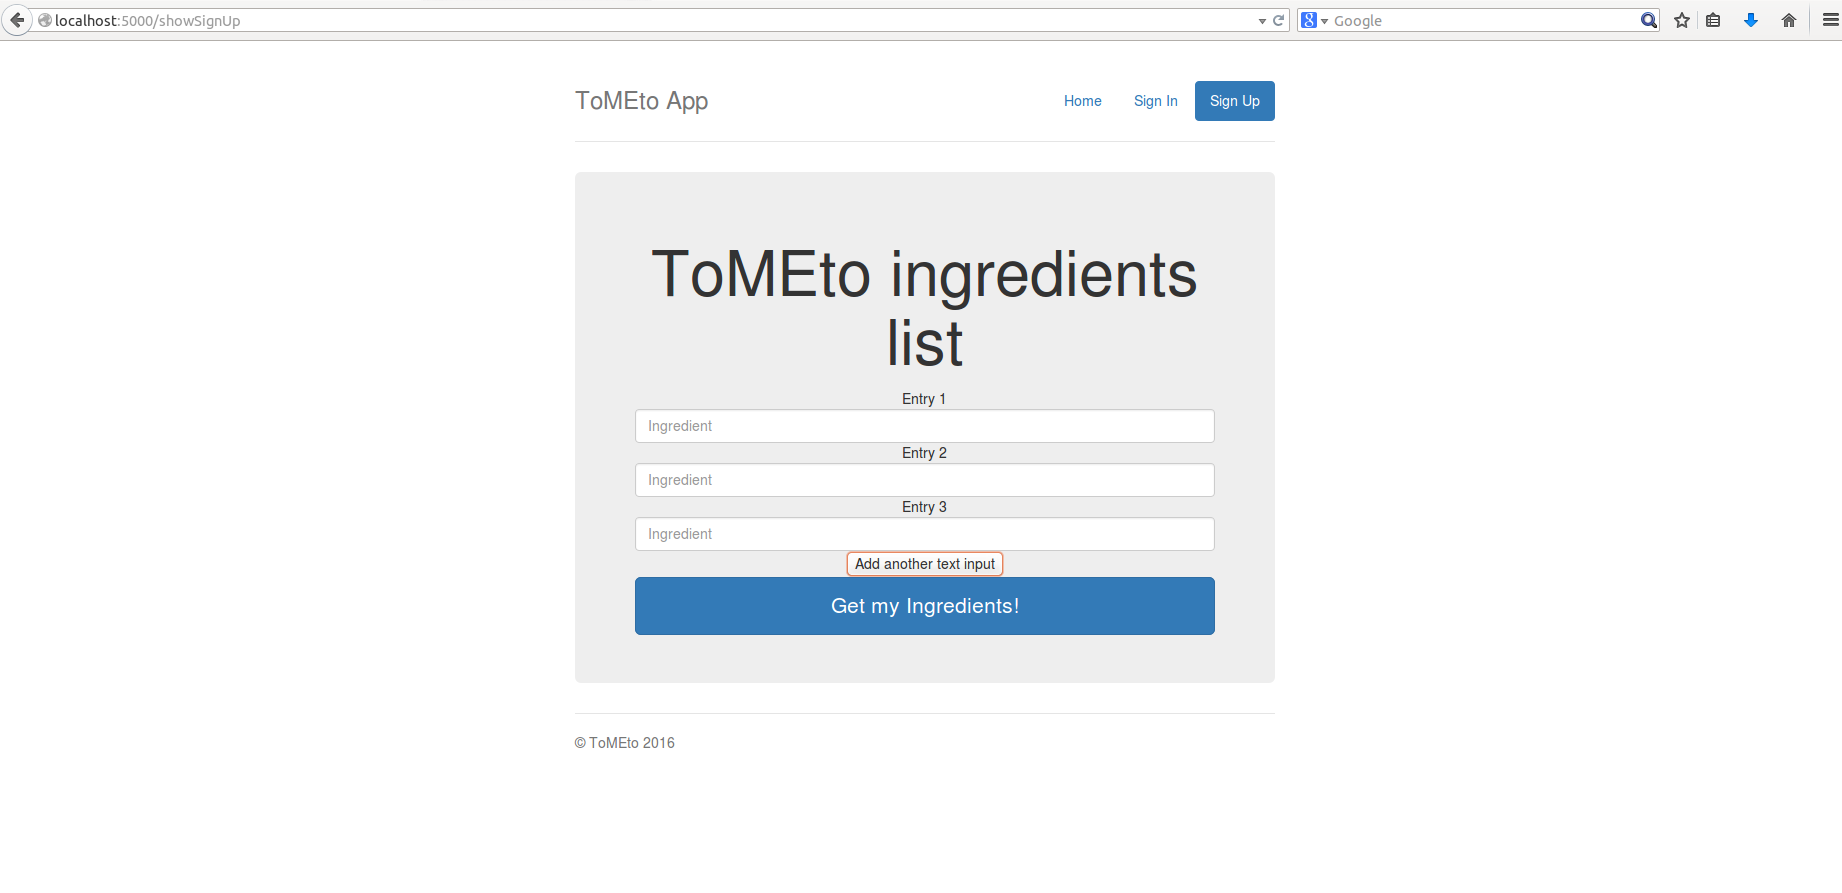
\includegraphics[scale=0.4]{secondpage.PNG}
\end{center}


The major challenge was learning about front-end development. Furthermore, while there existed sites which explained the implementation of certain features, it was difficult to determine how the existing code worked, and modify it as needed.

This basic layout is useful for testing purposes and offers a good foundation for the further development of our web application. From this, we know that integration of back-end and front-end should not be too much of an issue, as the large part of linking the two was accomplished with our test webpage.

TODO: As far as front-end, there is a lot that can be done to improve the overall look and feel of the webpage. Once we get a better idea of our target use cases, we can edit the formatting and the entry forms on our webpage to be more intuitive regarding the use case, as well as add some descriptions on what ToMEto actually does.



\section{Contributions}
\textbf{Jonathan Joo:} Front-end APIs (2.5)

\textbf{Matthew Jin:} Research on existing applications \& literature (2.1-2.2)

\textbf{Charlie Tong:} Data collection \& storage (2.4)

\textbf{Albert Ge:} Research on existing applications \& literature (2.1-2.2)



\section{Adjustments to plan}
We've realized the paper reading has and remains an integral source of inspiration for solidifying a use case. While we have certainly met our first biweekly milestone, paper reading will remain part of our work for future weeks, as we need to continue figuring out what analytical methods will work best for our data. 

\end{document}
